\gaokaoheader{2020}{江苏卷}

\gaokaoxz
\begin{enumerate}
%\renewcommand{\labelenumi}{\arabic{enumi}.}
% A(\Alph) a(\alph) I(\Roman) i(\roman) 1(\arabic)
%设定全局标号series=example	%引用全局变量resume=example
%[topsep=-0.3em,parsep=-0.3em,itemsep=-0.3em,partopsep=-0.3em]
%可使用leftmargin调整列表环境左边的空白长度 [leftmargin=0em]


%一、单项选择题:本题共5小题,每小题3分,共计15分.每小题只有一个选项符合题意.	

\item
质量为 $ 1.5 \times 10^{3} \ kg $ 的汽车在水平路面上匀速行驶,速度为 $ 20 \ m/s $,受到的阻力大小为 $ 1.8 \times 10^3 \ N $。此时,
汽车发动机输出的实际功率是 \xzanswer{C} 

\fourchoices
{$ 90 \ W $}
{$ 30 \ kW $}
{$ 36 \ kW $}
{$ 300 \ kW $}

%题目类型:选择
%题目难度:9.5
%题目区域:能量守恒:功与功率
%思想方法:
%题目特征:
%题目备注:



\item
电流互感器是一种测量电路中电流的变压器,工作原理如图所示.其原线圈匝数较少,串联在电路中,副
线圈匝数较多,两端接在电流表上.则电流互感器 \xzanswer{D} 
\begin{figure}[h!]
\centering
\includesvg[width=0.23\linewidth]{picture/svg/GZ-3-tiyou-0655}
\end{figure}


\fourchoices
{是一种降压变压器}
{能测量直流电路的电流}
{原、副线圈电流的频率不同}
{副线圈的电流小于原线圈的电流}

%题目类型:选择
%题目难度:9
%题目区域:电磁感应:变压器与高压输电
%思想方法:
%题目特征:
%题目备注:



\item
如图所示,两匀强磁场的磁感应强度 $ B_{1} $ 和 $ B_{2} $ 大小相等、方向相反.金属圆环的直径与两磁场的边界重合.
下列变化会在环中产生顺时针方向感应电流的是 \xzanswer{B} 
\begin{figure}[h!]
\centering
\includesvg[width=0.23\linewidth]{picture/svg/GZ-3-tiyou-0656}
\end{figure}


\fourchoices
{同时增大 $ B_{1} $ 减小 $ B_{2} $}
{同时减小 $ B_{1} $ 增大 $ B_{2} $}
{同时以相同的变化率增大 $ B_{1} $ 和 $ B_{2} $}
{同时以相同的变化率减小 $ B_{1} $ 和 $ B_{2} $}

%题目类型:选择
%题目难度:7.5
%题目区域:电磁感应:楞次定律
%思想方法:
%题目特征:
%题目备注:



\item
如图所示,一小物块由静止开始沿斜面向下滑动,最后停在水平地面上.斜面和地面平滑连接,且物块与
斜面、物块与地面间的动摩擦因数均为常数.该过程中,物块的动能 $ E_{k} $ 与水平位移 $ x $ 关系的图象是 \xzanswer{A} 
\begin{figure}[h!]
\centering
\includesvg[width=0.3\linewidth]{picture/svg/GZ-3-tiyou-0657}
\end{figure}

\pfourchoices
{\includesvg[width=3cm]{picture/svg/GZ-3-tiyou-0658}}
{\includesvg[width=3cm]{picture/svg/GZ-3-tiyou-0659}}
{\includesvg[width=3cm]{picture/svg/GZ-3-tiyou-0660}}
{\includesvg[width=3cm]{picture/svg/GZ-3-tiyou-0661}}



%题目类型:选择
%题目难度:6
%题目区域:能量守恒:动能定理
%思想方法:
%题目特征:图像选择
%题目备注:




\item
中欧班列在欧亚大陆开辟了“生命之路”
,为国际抗疫贡献了中国力量.某运送防疫物资的班列由 $ 40 $ 节质
量相等的车厢组成,在车头牵引下,列车沿平直轨道匀加速行驶时,第 $ 2 $ 节对第 $ 3 $ 节车厢的牵引力为 $ F $.若
每节车厢所受摩擦力、空气阻力均相等,则倒数第 $ 3 $ 节对倒数第 $ 2 $ 节车厢的牵引力为 \xzanswer{C} 

\fourchoices
{$F$}
{$\frac{19 F}{20}$}
{$\frac{F}{19}$}
{$\frac{F}{20}$}

%题目类型:选择
%题目难度:5
%题目区域:运动定律:牛二律
%思想方法:
%题目特征:材料分析
%题目备注:



%二、多项选择题:本题共 $ 4 $ 小题,每小题 $ 4 $ 分,共计 $ 16 $ 分.每小题有多个选项符合题意.全部选对的得 $ 4 $ 分,选对但不全的得 $ 2 $ 分,错选或不答的得 $ 0 $ 分.


\item
某汽车的电源与启动电机、车灯连接的简化电路如图所示.当汽车启动时,开关 $ S $ 闭合,电机工作,车灯
突然变暗,此时\xzanswer{ABD} 
\begin{figure}[h!]
\centering
\includesvg[width=0.26\linewidth]{picture/svg/GZ-3-tiyou-0662}
\end{figure}


\fourchoices
{车灯的电流变小}
{路端电压变小}
{电路的总电流变小}
{电源的总功率变大}

%题目类型:选择
%题目难度:6
%题目区域:电路
%思想方法:
%题目特征:
%题目备注:




\item
甲、乙两颗人造卫星质量相等,均绕地球做圆周运动,甲的轨道半径是乙的 $ 2 $ 倍.下列应用公式进行的推
论正确的有 \xzanswer{CD} 

\fourchoices
{由 $v=\sqrt{g R}$ 可知,甲的速度是乙的 $\sqrt{2}$ 倍}
{由 $a=\omega^{2} r$ 可知,甲的向心加速度是乙的 2 倍}
{由$ F=G \frac{M m}{r^{2}}$ 可知,甲的向心力是乙的 $\frac{1}{4}$}
{由 $\frac{r^{3}}{T^{2}}=k$ 可知,甲的周期是乙的 $2 \sqrt{2}$ 倍}


%题目类型:选择
%题目难度:7
%题目区域:万有引力
%思想方法:
%题目特征:
%题目备注:




\item 
如图所示,小球 $ A $、$ B $ 分别从 $ 2l $ 和 $ l $ 的高度水平抛出后落地,上述过程中 $ A $、$ B $ 的水平位移分别为 $ l $ 和 $ 2l $.
忽略空气阻力,则 \xzanswer{AD} 
\begin{figure}[h!]
\centering
\includesvg[width=0.23\linewidth]{picture/svg/GZ-3-tiyou-0663}
\end{figure}


\fourchoices
{$ A $ 和 $ B $ 的位移大小相等}
{$ A $ 的运动时间是 $ B $ 的 $ 2 $ 倍}
{$ A $ 的初速度是 $ B $ 的$ \frac{ 1 }{ 2 } $}
{$ A $ 的末速度比 $ B $ 的大}

%题目类型:选择
%题目难度:5.5
%题目区域:曲线运动:平抛
%思想方法:
%题目特征:
%题目备注:




\item
如图所示,绝缘轻杆的两端固定带有等量异号电荷的小球(不计重力)。开始时,两小球分别静止在 $ A $、$ B $
位置.现外加一匀强电场 $ E $,在静电力作用下,小球绕轻杆中点 $ O $ 转到水平位置.取 $ O $ 点的电势为 $ 0 $.下列说法
正确的有 \xzanswer{AB} 
\begin{figure}[h!]
\centering
\includesvg[width=0.23\linewidth]{picture/svg/GZ-3-tiyou-0664}
\end{figure}


\fourchoices
{电场 $ E $ 中 $ A $ 点电势低于 $ B $ 点}
{转动中两小球的电势能始终相等}
{该过程静电力对两小球均做负功}
{该过程两小球的总电势能增加}

%题目类型:选择
%题目难度:6
%题目区域:电场:电势能
%思想方法:
%题目特征:
%题目备注:





%三、简答题:本题分必做题(第 $ 10 \sim 12 $ 题)和选做题(第 $ 13 $ 题)两部分,共计 $ 42 $ 分.请将解答填写在答题卡相应的位置.
%【必做题】

\gaokaosy

\item
某同学描绘一种电子元件的 $ I-U $ 关系图象,采用的实验电路图如图$ a $所示,$ \voltmetermytikz $ 为电压表,  
$ \mammetermytikz $    为电流表,$ E $ 为电源(电动势约 $ 6 \ V $ ),$ R $ 为滑动变阻器(最大阻值 $ 20 \ \Omega $ ), $ R_{0} $ 为定值电阻,$ S $ 为开关。

\begin{enumerate}
%\renewcommand{\labelenumi}{\arabic{enumi}.}
% A(\Alph) a(\alph) I(\Roman) i(\roman) 1(\arabic)
%设定全局标号series=example	%引用全局变量resume=example
%[topsep=-0.3em,parsep=-0.3em,itemsep=-0.3em,partopsep=-0.3em]
%可使用leftmargin调整列表环境左边的空白长度 [leftmargin=0em]
\item
请用笔画线代替导线,将图$ b $所示的实物电路连接完整.
\begin{figure}[h!]
\centering
\begin{subfigure}{0.4\linewidth}
\centering
\includesvg[width=0.7\linewidth]{picture/svg/GZ-3-tiyou-0665} 
\caption{}\label{}
\end{subfigure}
\begin{subfigure}{0.4\linewidth}
\centering
\includesvg[width=0.8\linewidth]{picture/svg/GZ-3-tiyou-0667} 
\caption{}\label{}
\end{subfigure}

\end{figure}

\newpage

\item 
调节滑动变阻器,记录电压表和电流表的示数如下表:

\begin{table}[h!]
\centering 
\begin{tabular}{|c|c|c|c|c|c|c|c|}
\hline 
电压$ U/V $ & 0.000 & 0.250 & 0.500 & 0.650 & 0.700 & 0.725 & 0.750
\\
\hline
电流$ I/mA $ & 0.00 & 0.10 & 0.25 & 0.60 & 1.70 & 4.30 & 7.50\\ 
\hline 
\end{tabular}
\end{table} 




请根据表中的数据,在方格纸上作出该元件的 $ I-U $ 图线.

\begin{figure}[h!]
	\centering
%\includesvg[width=0.5\linewidth]{picture/svg/GZ-3-tiyou-0668}
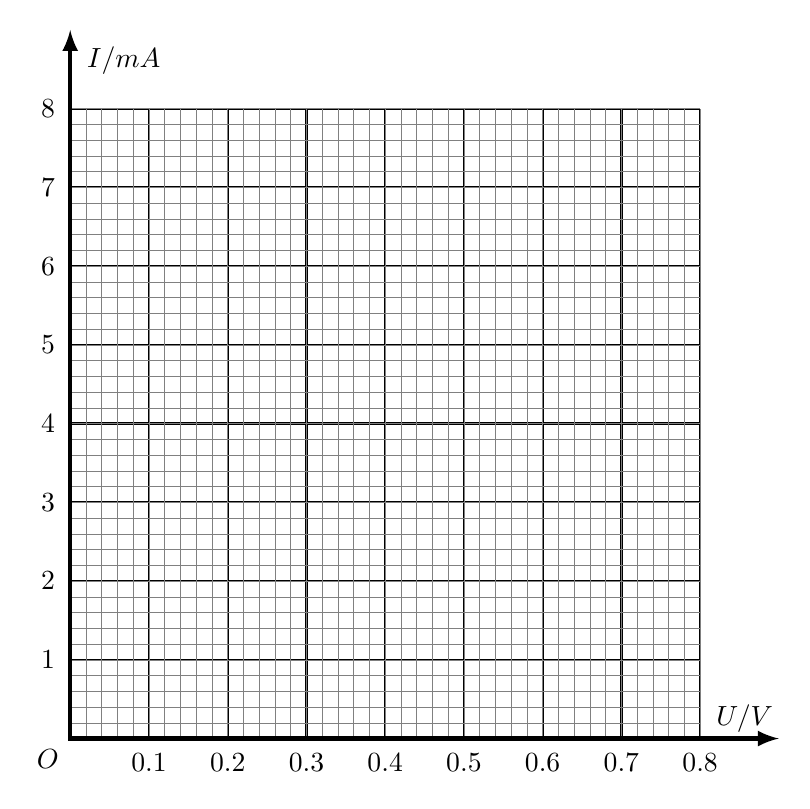
\begin{tikzpicture}
%网格
	\draw[thick] (0,0) grid (8,8);
	\draw[step=0.2cm,gray,very thin] (0,0) grid (8,8);

%坐标轴
	\draw[ultra thick,latex-latex] (9,0) node [above left=-2pt] {$ U/V $} --  (0,0) node [below left ] {$ O $}   -- (0,9) node [below right=2pt] {$ I/mA $} ;



%刻度
	\foreach \label in {1,2,...,8}
	{
\node[below=2pt]  (ww) at (\label cm , 0) {$ 0.\label $}	;
\node[left=2pt]  (ww) at (0, \label cm) {$ \label $}	;
}


\end{tikzpicture}
\end{figure}

\item 
根据作出的 $ I-U $ 图线可知,该元件是 \underlinegap (选填“线性”或“非线性”)元件.
\item 
在上述测量中,如果用导线代替电路中的定值电阻 $ R_{0} $,会导致的两个后果是 \underlinegap 。
\fourchoices
{电压和电流的测量误差增大}
{可能因电流过大烧坏待测元件}
{滑动变阻器允许的调节范围变小}
{待测元件两端电压的可调节范围变小}


\end{enumerate}


\tk{
\begin{enumerate}
%\renewcommand{\labelenumi}{\arabic{enumi}.}
% A(\Alph) a(\alph) I(\Roman) i(\roman) 1(\arabic)
%设定全局标号series=example	%引用全局变量resume=example
%[topsep=-0.3em,parsep=-0.3em,itemsep=-0.3em,partopsep=-0.3em]
%可使用leftmargin调整列表环境左边的空白长度 [leftmargin=0em]
\item
如图
\begin{center}
\includesvg[width=0.93\linewidth]{picture/svg/GZ-3-tiyou-0675} 
\end{center}
\item 
如图
\begin{center}
\includesvg[width=0.93\linewidth]{picture/svg/GZ-3-tiyou-0676} 
\end{center}
\item 
非线性
\item 
BC
\end{enumerate}
} 

%题目类型:实验
%题目难度:7.5
%题目区域:电路
%思想方法:
%题目特征:
%题目备注:




\item
疫情期间“停课不停学”
,小明同学在家自主开展实验探究.用手机拍摄物体自由下落的视频,
得到分帧图片,利用图片中小球的位置来测量当地的重力加速度,实验装置如图$ a $所示.
\begin{figure}[h!]
\centering
\begin{subfigure}{0.35\linewidth}
\centering
\includesvg[width=0.7\linewidth]{picture/svg/GZ-3-tiyou-0669} 
\caption{}\label{}
\end{subfigure}
\begin{subfigure}{0.55\linewidth}
\centering
\includesvg[width=0.96\linewidth]{picture/svg/GZ-3-tiyou-0670} 
\caption{}\label{}
\end{subfigure}
\end{figure}
\begin{enumerate}
%\renewcommand{\labelenumi}{\arabic{enumi}.}
% A(\Alph) a(\alph) I(\Roman) i(\roman) 1(\arabic)
%设定全局标号series=example	%引用全局变量resume=example
%[topsep=-0.3em,parsep=-0.3em,itemsep=-0.3em,partopsep=-0.3em]
%可使用leftmargin调整列表环境左边的空白长度 [leftmargin=0em]
\item
家中有乒乓球、小塑料球和小钢球,其中最适合用作实验中下落物体的是 \underlinegap .
\item 
下列主要操作步骤的正确顺序是 \underlinegap .(填写各步骤前的序号)

①把刻度尺竖直固定在墙上

②捏住小球,从刻度尺旁静止释放

③手机固定在三角架上,调整好手机镜头的位置

④打开手机摄像功能,开始摄像

\item 
停止摄像,从视频中截取三帧图片,图片中的小球和刻度如图$ 2 $所示.已知所截取的图片相邻两
帧之间的时间间隔为 $ \frac{ 1 }{ 6 } \ s $,刻度尺的分度值是 $ 1 \ mm $,由此测得重力加速度为 \underlinegap $ m/s^{2} $.

\item 
在某次实验中,小明释放小球时手稍有晃动,视频显示小球下落时偏离了竖直方向.从该视频中截取图
片, \underlinegap (选填“仍能”或“不能”)用($ 3 $)问中的方法测出重力加速度.

\end{enumerate}


\tk{
\begin{enumerate}
%\renewcommand{\labelenumi}{\arabic{enumi}.}
% A(\Alph) a(\alph) I(\Roman) i(\roman) 1(\arabic)
%设定全局标号series=example	%引用全局变量resume=example
%[topsep=-0.3em,parsep=-0.3em,itemsep=-0.3em,partopsep=-0.3em]
%可使用leftmargin调整列表环境左边的空白长度 [leftmargin=0em]
\item
小钢球 
\item 
①③④② 
\item 
$ 9.6 $($ 9.5 \sim 9.7 $都算对) 
\item 
仍能	
\end{enumerate}
} 


%题目类型:实验
%题目难度:7
%题目区域:直线运动
%思想方法:
%题目特征:
%题目备注:






\gaokaoxx{$ 3-5 $}



\item 
%选修 $ 3-5 $
\begin{enumerate}
%\renewcommand{\labelenumi}{\arabic{enumi}.}
% A(\Alph) a(\alph) I(\Roman) i(\roman) 1(\arabic)
%设定全局标号series=example	%引用全局变量resume=example
%[topsep=-0.3em,parsep=-0.3em,itemsep=-0.3em,partopsep=-0.3em]
%可使用leftmargin调整列表环境左边的空白长度 [leftmargin=0em]
\item
“测温枪”
(学名“红外线辐射测温仪”)具有响应快、非接触和操作方便等优点.它是根据黑体辐射规
律设计出来的,能将接收到的人体热辐射转换成温度显示.若人体温度升高,则人体热辐射强度 $ I $ 及其极大
值对应的波长 $ \lambda $ 的变化情况是 \underlinegap .
\fourchoices
{$ I $增大, $ \lambda $ 增大}
{$ I $ 增大, $ \lambda $ 减小}
{$ I $ 减小, $ \lambda $ 增大}
{$ I $ 减小, $ \lambda $ 减小}

\tk{B} 


%题目类型:选择
%题目难度:7.5
%题目区域:电磁波:原子物理
%思想方法:
%题目特征:材料分析
%题目备注:



\item 
大量处于某激发态的氢原子辐射出多条谱线,其中最长和最短波长分别为 $ \lambda_{1} $ 和 $ \lambda_{2} $,则该激发态与基
态的能量差为 \underlinegap ,波长为 $ \lambda_{1} $ 的光子的动量为 \underlinegap .(已知普朗克常量为 $ h $,光速为 $ c $)

\tk{$\frac{h c}{\lambda_{2}} \quad \frac{h}{\lambda_{1}}$} 


%题目类型:填空
%题目难度:8
%题目区域:原子物理
%思想方法:
%题目特征:
%题目备注:



\item 
一只质量为 $ 1.4 \ kg $ 的乌贼吸入 $ 0.1 \ kg $ 的水,静止在水中.遇到危险时,它在极短时间内把吸入的水向后
全部喷出,以 $ 2 \ m/s $ 的速度向前逃窜.求该乌贼喷出的水的速度大小 $ v $.

\banswer{
$v=28 \ m / s$
}

%题目类型:计算
%题目难度:8.5
%题目区域:动量:动量守恒
%思想方法:
%题目特征:
%题目备注:




\end{enumerate}





%【选做题】


%13.本题包括 $ A $、$ B $ 两小题,请选定其中一小题,并在相应的答题区域内作答.若多做,则按 $ A $ 小题评分.


\newpage

\gaokaoxx{$ 3-3 $}

\item 
%选修 $ 3-3 $
\begin{enumerate}
%\renewcommand{\labelenumi}{\arabic{enumi}.}
% A(\Alph) a(\alph) I(\Roman) i(\roman) 1(\arabic)
%设定全局标号series=example	%引用全局变量resume=example
%[topsep=-0.3em,parsep=-0.3em,itemsep=-0.3em,partopsep=-0.3em]
%可使用leftmargin调整列表环境左边的空白长度 [leftmargin=0em]
\item
玻璃的出现和使用在人类生活里已有四千多年的历史,它是一种非晶体.下列关于玻璃的说法正确的有 \underlinegap .
\fourchoices
{没有固定的熔点}
{天然具有规则的几何形状}
{沿不同方向的导热性能相同}
{分子在空间上周期性排列}

\tk{AC} 

%题目类型:选择
%题目难度:8
%题目区域:分子动理论
%思想方法:
%题目特征:
%题目备注:




\item 
一瓶酒精用了一些后,把瓶盖拧紧,不久瓶内液面上方形成了酒精的饱和汽,此时 \underlinegap (选填“有”
或“没有”
)酒精分子从液面飞出.当温度升高时,瓶中酒精饱和汽的密度 \underlinegap (选填“增大”
“减小”或“不
变”).

\tk{有 \quad 增大} 


%题目类型:填空
%题目难度:8
%题目区域:分子动理论
%思想方法:
%题目特征:
%题目备注:



\item 
一定质量的理想气体从状态 $ A $ 经状态 $ B $ 变化到状态 $ C $,其 $ p-\frac{1}{V} $
图象如图所示,求该过程中气体吸收
的热量 $ Q $.
\begin{figure}[h!]
\flushright
\includesvg[width=0.25\linewidth]{picture/svg/GZ-3-tiyou-0671}
\end{figure}

\banswer{
$Q=2 \times 10^{5} \ J$
}


%题目类型:计算
%题目难度:5.5
%题目区域:热学:热力学第一定律:理想气体状态方程
%思想方法:
%题目特征:图像分析
%题目备注:



\end{enumerate}




\gaokaoxx{$ 3-4 $}



\item 

%选修 $ 3-4 $
\begin{enumerate}
%\renewcommand{\labelenumi}{\arabic{enumi}.}
% A(\Alph) a(\alph) I(\Roman) i(\roman) 1(\arabic)
%设定全局标号series=example	%引用全局变量resume=example
%[topsep=-0.3em,parsep=-0.3em,itemsep=-0.3em,partopsep=-0.3em]
%可使用leftmargin调整列表环境左边的空白长度 [leftmargin=0em]
\item
电磁波广泛应用在现代医疗中.下列属于电磁波应用的医用器械有 \underlinegap .
\fourchoices
{杀菌用的紫外灯}
{拍胸片的 $ X $ 光机}
{治疗咽喉炎的超声波雾化器}
{检查血流情况的“彩超”机}

\tk{AB} 


%题目类型:选择
%题目难度:7.5
%题目区域:电磁波
%思想方法:
%题目特征:
%题目备注:



\item 
我国的光纤通信技术处于世界领先水平.光纤内芯(内层玻璃)的折射率比外套(外层玻璃)的
\underlinegap (选填“大”或“小”
).某种光纤的内芯在空气中全反射的临界角为 $ 43 ^{ \circ } $,则该内芯的折射率为 \underlinegap .(取
$ \sin 43 ^{ \circ } =0.68, \cos 43 ^{ \circ } =0.73 $,结果保留 $ 2 $ 位有效数字)


\tk{大 \quad 1.5} 


%题目类型:实验
%题目难度:6
%题目区域:光学:光的折射
%思想方法:
%题目特征:
%题目备注:



\item 
国际宇航联合会将 $ 2020 $ 年度“世界航天奖”授予我国“嫦娥四号”任务团队.“嫦娥四号”任务创造
了多项世界第一.在探月任务中,
“玉兔二号”月球车朝正下方发射一束频率为 $ f $ 的电磁波,该电磁波分别在
月壤层的上、下表面被反射回来,反射波回到“玉兔二号”的时间差为 $ \Delta t $.已知电磁波在月壤层中传播的波
长为 $ \lambda $,求该月壤层的厚度 $ d $.

\banswer{
$d=\frac{f \lambda \Delta t}{2}$
}

%题目类型:计算
%题目难度:7
%题目区域:电磁波
%思想方法:
%题目特征:
%题目备注:




\end{enumerate}



\gaokaojs

%四、计算题:本题共 $ 3 $ 小题,共计 $ 47 $ 分.解答时请写出必要的文字说明、方程式和重要的演算步骤.只写出最后答案的不能得分.有数值计算的题,答案中必须明确写出数值和单位.


\item
如图所示,电阻为 $ 0.1 \ \Omega $ 的正方形单匝线圈 $ abcd $ 的边长为 $ 0.2 \ m $, $ bc $ 边与匀强磁场边缘重合.
磁场的宽度等于线圈的边长,磁感应强度大小为 $ 0.5 \ T $.在水平拉力作用下,线圈以 $ 8 \ m/s $ 的速度向右穿过磁
场区域.求线圈在上述过程中:
\begin{enumerate}
%\renewcommand{\labelenumi}{\arabic{enumi}.}
% A(\Alph) a(\alph) I(\Roman) i(\roman) 1(\arabic)
%设定全局标号series=example	%引用全局变量resume=example
%[topsep=-0.3em,parsep=-0.3em,itemsep=-0.3em,partopsep=-0.3em]
%可使用leftmargin调整列表环境左边的空白长度 [leftmargin=0em]
\item
感应电动势的大小 $ E $;
\item 
所受拉力的大小 $ F $;
\item 
感应电流产生的热量 $ Q $.

\end{enumerate}
\begin{figure}[h!]
\flushright
\includesvg[width=0.33\linewidth]{picture/svg/GZ-3-tiyou-0672}
\end{figure}

\banswer{
\begin{enumerate}
%\renewcommand{\labelenumi}{\arabic{enumi}.}
% A(\Alph) a(\alph) I(\Roman) i(\roman) 1(\arabic)
%设定全局标号series=example	%引用全局变量resume=example
%[topsep=-0.3em,parsep=-0.3em,itemsep=-0.3em,partopsep=-0.3em]
%可使用leftmargin调整列表环境左边的空白长度 [leftmargin=0em]
\item
$E=0.8 \ V$	
\item 	
$F=0.8 \ N$
\item 
$Q=0.32 \ J$	
\end{enumerate}
}

%题目类型:计算
%题目难度:7
%题目区域:电磁感应:电磁感应定律:磁场:安培力
%思想方法:
%题目特征:
%题目备注:




\item
如图所示,鼓形轮的半径为 $ R $,可绕固定的光滑水平轴 $ O $ 转动.在轮上沿相互垂直的直径方向固
定四根直杆,杆上分别固定有质量为 $ m $ 的小球,球与 $ O $ 的距离均为 $ 2R $.在轮上绕有长绳,绳上悬挂着质量
为 $ M $ 的重物.重物由静止下落,带动鼓形轮转动.重物落地后鼓形轮匀速转动,转动的角速度为 $ \omega $.绳与轮之
间无相对滑动,忽略鼓形轮、直杆和长绳的质量,不计空气阻力,重力加速度为 $ g $.求:
\begin{enumerate}
%\renewcommand{\labelenumi}{\arabic{enumi}.}
% A(\Alph) a(\alph) I(\Roman) i(\roman) 1(\arabic)
%设定全局标号series=example	%引用全局变量resume=example
%[topsep=-0.3em,parsep=-0.3em,itemsep=-0.3em,partopsep=-0.3em]
%可使用leftmargin调整列表环境左边的空白长度 [leftmargin=0em]
\item
重物落地后,小球线速度的大小 $ v $;
\item 
重物落地后一小球转到水平位置 $ A $,此时该球受到杆的作用力的大小 $ F $;
\item 
重物下落的高度 $ h $.
\end{enumerate}
\begin{figure}[h!]
\flushright
\includesvg[width=0.25\linewidth]{picture/svg/GZ-3-tiyou-0673}
\end{figure}



\banswer{
\begin{enumerate}
%\renewcommand{\labelenumi}{\arabic{enumi}.}
% A(\Alph) a(\alph) I(\Roman) i(\roman) 1(\arabic)
%设定全局标号series=example	%引用全局变量resume=example
%[topsep=-0.3em,parsep=-0.3em,itemsep=-0.3em,partopsep=-0.3em]
%可使用leftmargin调整列表环境左边的空白长度 [leftmargin=0em]
\item
$v=2 \omega R$	
\item 
$F=\sqrt{\left(2 m \omega^{2} R\right)^{2}+(m g)^{2}}$
\item 
$h=\frac{M+16 m}{2 M g}(\omega R)^{2}$
\end{enumerate}
}

%题目类型:计算
%题目难度:6.5
%题目区域:能量守恒:曲线运动:圆周
%思想方法:
%题目特征:材料分析
%题目备注:





\newpage

\item
空间存在两个垂直于 $ Oxy $ 平面的匀强磁场,$ y $ 轴为两磁场的边界,磁感应强度分别为 $ 2B_{0} $、$ 3B_{0} $.
甲、乙两种比荷不同的粒子同时从原点 $ O $ 沿 $ x $ 轴正向射入磁场,速度均为 $ v $.甲第 $ 1 $ 次、第 $ 2 $ 次经过 $ y $ 轴的
位置分别为 $ P $、$ Q $,其轨迹如图所示.甲经过 $ Q $ 时,乙也恰好同时经过该点.已知甲的质量为 $ m $,电荷量为 $ q $.
不考虑粒子间的相互作用和重力影响.求:
\begin{enumerate}
%\renewcommand{\labelenumi}{\arabic{enumi}.}
% A(\Alph) a(\alph) I(\Roman) i(\roman) 1(\arabic)
%设定全局标号series=example	%引用全局变量resume=example
%[topsep=-0.3em,parsep=-0.3em,itemsep=-0.3em,partopsep=-0.3em]
%可使用leftmargin调整列表环境左边的空白长度 [leftmargin=0em]
\item
$ Q $ 到 $ O $ 的距离 $ d $;
\item 
甲两次经过 $ P $ 点的时间间隔 $ \Delta t $;
\item 
乙的比荷$ \frac{q}{m} $可能的最小值.
\end{enumerate}
\begin{figure}[h!]
\flushright
\includesvg[width=0.28\linewidth]{picture/svg/GZ-3-tiyou-0674}
\end{figure}



\banswer{
\begin{enumerate}
%\renewcommand{\labelenumi}{\arabic{enumi}.}
% A(\Alph) a(\alph) I(\Roman) i(\roman) 1(\arabic)
%设定全局标号series=example	%引用全局变量resume=example
%[topsep=-0.3em,parsep=-0.3em,itemsep=-0.3em,partopsep=-0.3em]
%可使用leftmargin调整列表环境左边的空白长度 [leftmargin=0em]
\item
$d=\frac{m v}{3 q B_{0}}$
\item 
$\Delta t=\frac{2 \pi m}{q B_{0}}$
\item 
比荷的最小值为 $\frac{2 q}{m}$
\end{enumerate}
}

%题目类型:计算
%题目难度:5
%题目区域:磁场:磁场中带电粒子的运动
%思想方法:
%题目特征:计算练习
%题目备注:




\end{enumerate}

